\section{Hardware}

The robot used in this work is a modified version of the Turtlebot 2. The Yujin Kobuki base of the Turtlebot is a differential drive base with an odometry amended by a gyroscope. The maximum translational velocity of this base is 0.7 m/s and the maximum rotational velocity is 180°/s, though the full speed is not used. The maximum payload is 5 kg which is about the weight of the notebook and the construction.

For accurate localization and 2D mapping a Hokuyo laser range finders (LIDAR) is mounted on the base at a height of about 15 cm. The specified range is from 0.02 m to 4 m with an accuracy of $\pm10$ mm and the angular range is from -120° to 120° with a resolution of 0.36°. The LIDAR scans at a rate of 10 Hz.

The main camera for object detection, place classification and 3D mapping is an ASUS Xtion PRO LIVE RGBD-camera mounted at a height of about 1m facing slightly downwards. The camera takes color images and depth images at a rate of 30 Hz with a resolution of 640x480. The field of view is 58° horizontally and 45° vertically. The range of the depth measurements is specified with 0.8 m to 3.5 m, though experiments showed a minimum range of about 0.55 m. The accuracy of the depth image depends on many factors, especially on the distance and is somewhere around $\pm$5 cm (TODO genauer wert und referenz).\newline
For the detection of doorways another ASUS Xtion PRO LIVE was added looking upwards.

A Clevo notebook is mounted on the robot running the complete software with a $4^{th}$ generation Intel i7 quadcore CPU running at 2.4 GHz, 8 GB DDR3 RAM and a NVidia Geforce GT 750M GPU with 2 GB memory. 

Figure \ref{robot images} shows the robot and its dimensions, figure \ref{robot view} the sensor setup.

\begin{figure}[h]
  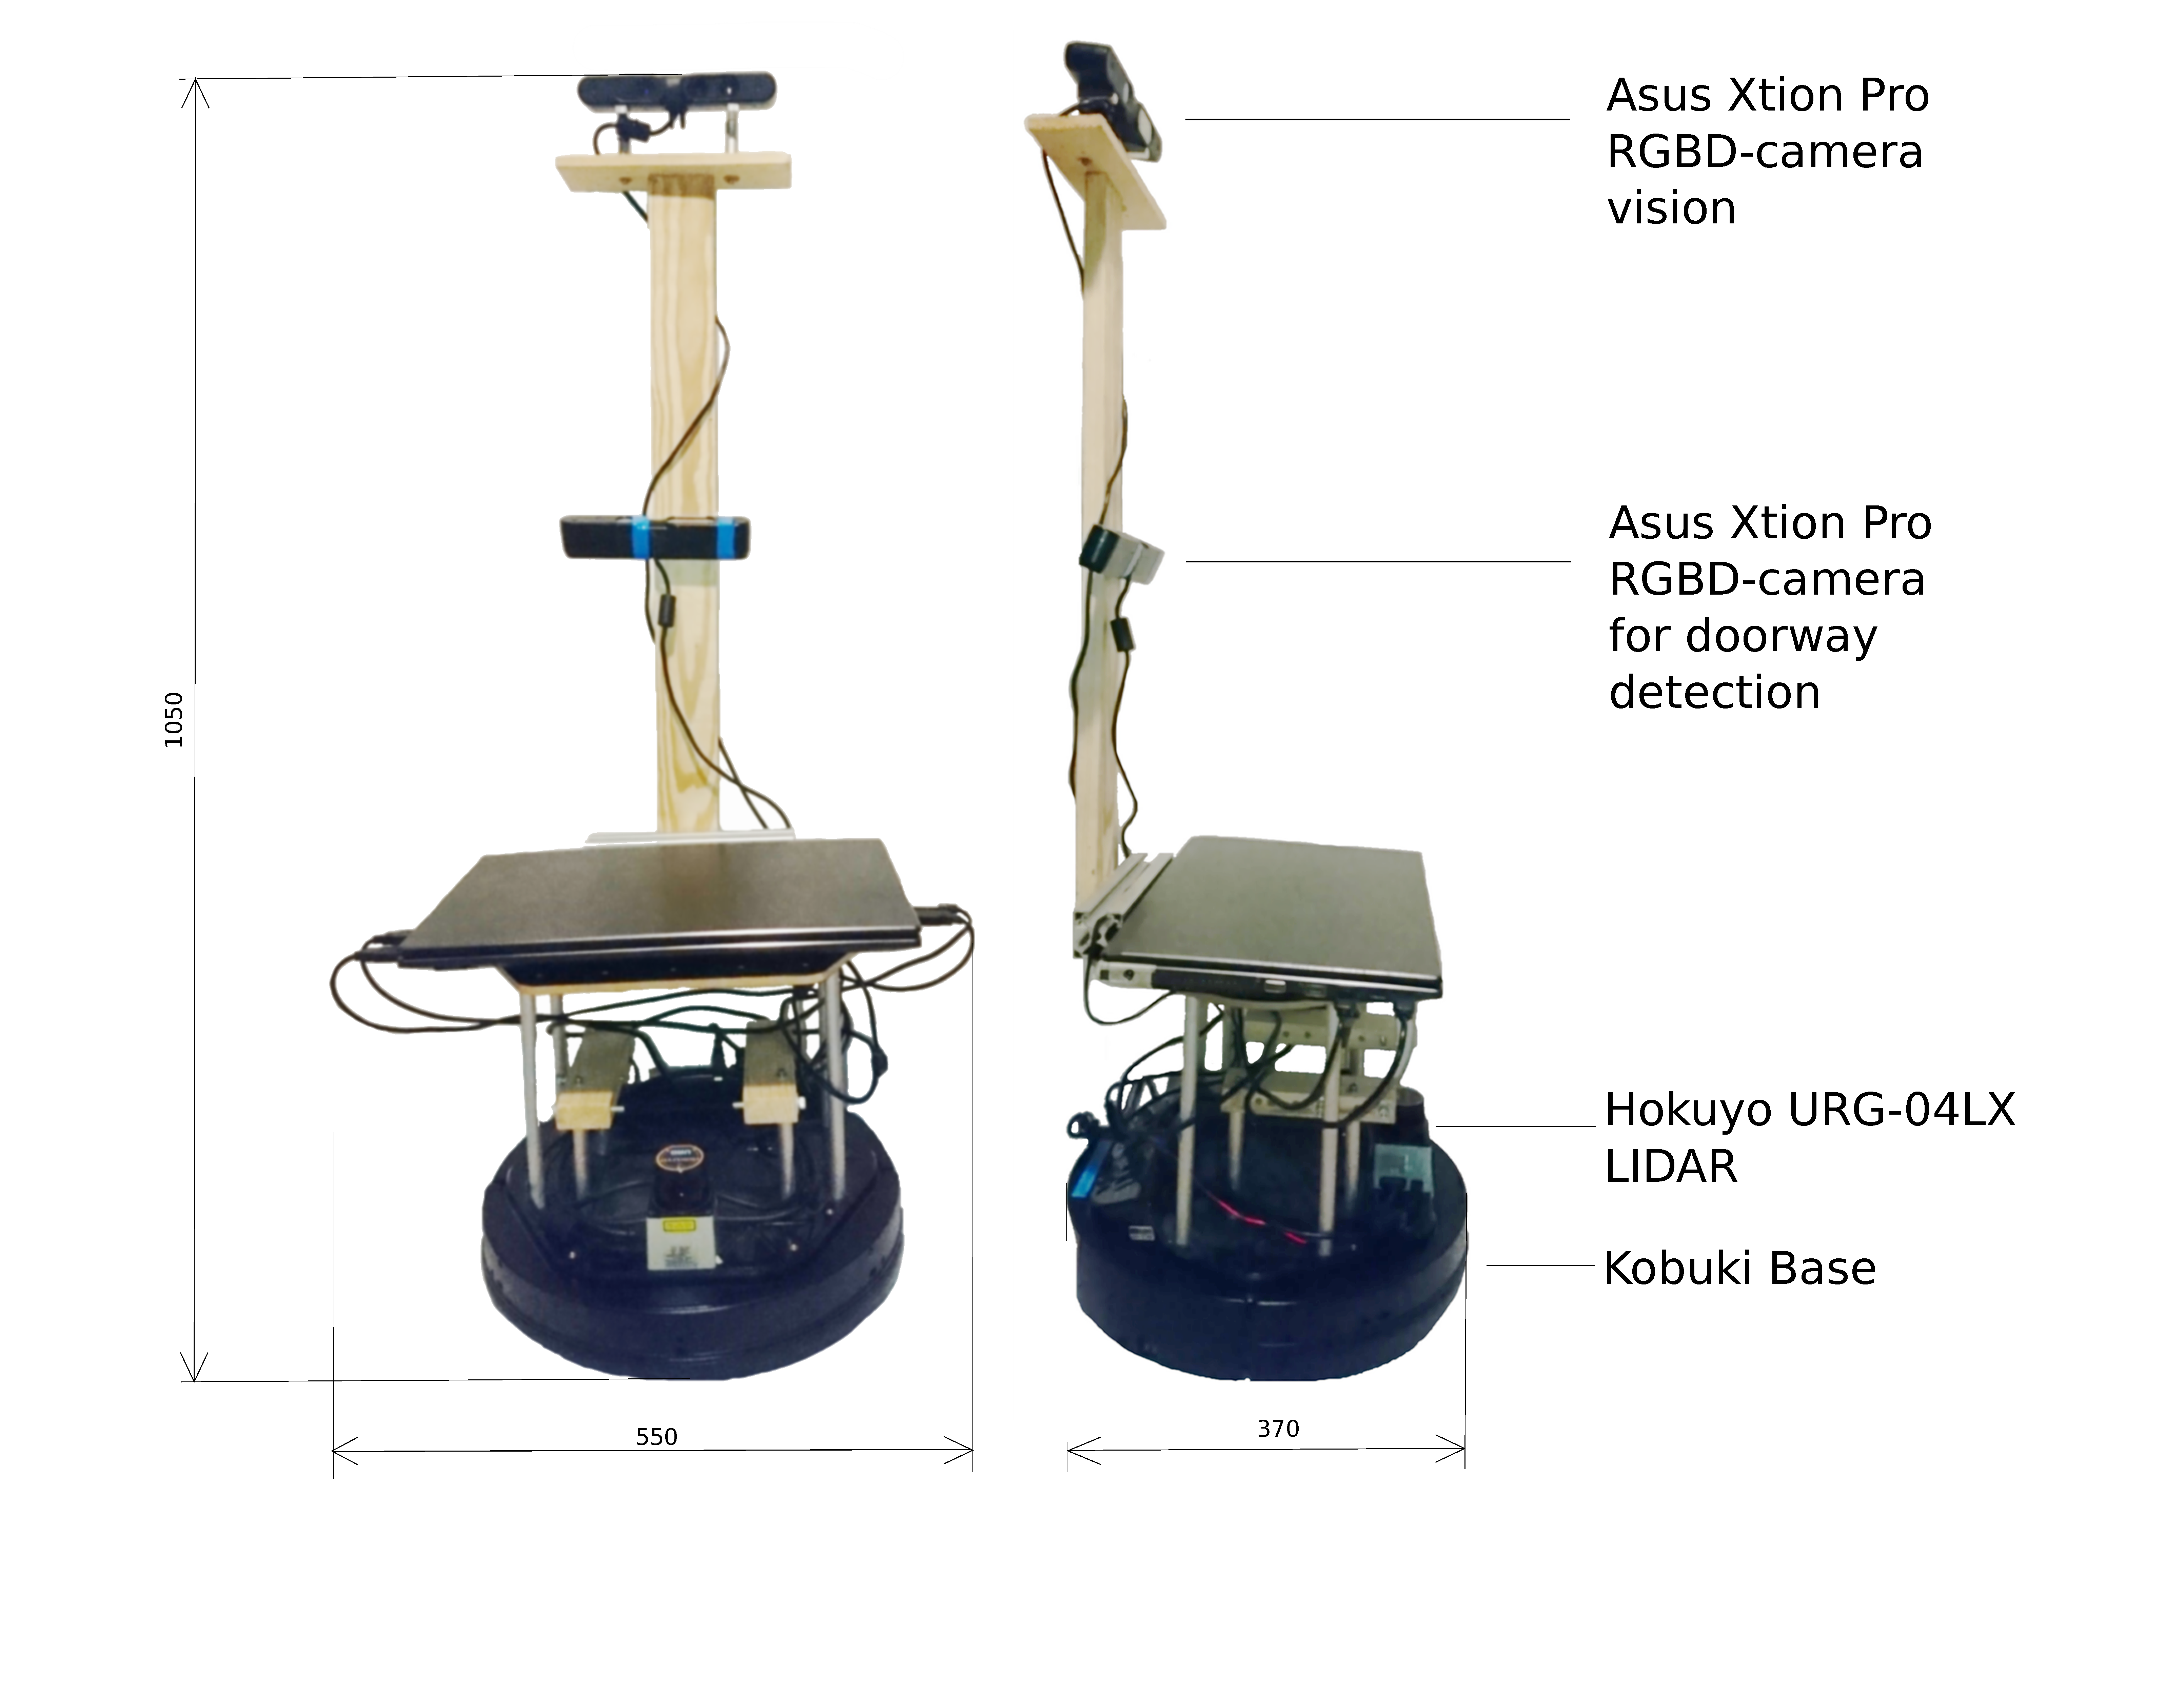
\includegraphics[width=1.02\textwidth,trim={0 10cm 0 0},clip]{figures/front_and_side.pdf}
  \caption{Robot setup in front and side view with labels of most important parts}
  \label{robot images}
\end{figure}

\begin{figure}[h]
  \includegraphics[width=1.0\textwidth]{figures/DSC_0032.JPG}
  \caption{Sensor setup of the robot}
  \label{robot view}
\end{figure}
